\documentclass[11pt,a4paper,fleqn,landscape]{scrartcl}
\usepackage[utf8]{inputenc}
\usepackage[english]{babel}
\usepackage{setspace}
\setstretch{0.9}
\usepackage{soul}	% highlighting
%--------------------------------Layout ------------------------------------
\usepackage{multicol}	% multiple columns
\usepackage{graphicx}	% images

\usepackage{todonotes}
\usepackage{tabularx,ragged2e}
\usepackage{array, makecell}

\pagestyle{empty}	% no page numbers
% -------------------------Colors -----------------------------------------------
\usepackage{xcolor}						% color
\definecolor{imp}{RGB}{127, 0, 255}
\definecolor{imp2}{RGB}{0, 204, 102}
\definecolor{imp3}{RGB}{51, 153, 255}
\definecolor{highlight}{RGB}{189, 255, 255}



%--------------------------------Pseudocode------------------------------------------
\usepackage[linesnumbered, ruled]{algorithm2e}
\SetKwRepeat{Do}{do}{while} 					
\SetKwRepeat{DoUntil}{do}{until}
\SetKwRepeat{RepeatUntil}{repeat}{until}


%% ----- Text -----
%\usepackage[bitstream-charter]{mathdesign}		% packet that changes the math + text font
%\let\circledS\undefined % conflict
%
%\usepackage[t1]{sourcesanspro}
\usepackage[scaled=0.86]{helvet} 
\usepackage{mathptmx}
\usepackage[mathcal]{euscript}


\renewcommand\emph[1]{\sethlcolor{highlight}\hl{#1}}

%\renewcommand\rmdefault{phv}	% Set text font separately


\setlength\parindent{0pt}		% no indent after paragraph

\usepackage{enumitem}			% lists
\setlist{nosep}
\setlist[itemize]{leftmargin=1em}
\setlist[enumerate]{leftmargin=*}
\renewcommand{\labelitemii}{$\cdot$}
\renewcommand{\labelitemi}{-}
\renewcommand{\labelitemiii}{$\diamond$}


% sections
\usepackage{titlesec}





% ----------------------------- Text formatting
\usepackage{microtype}

\usepackage{parskip}
\setlength{\parskip}{0pt} %set space after paragraph
%\setcounter{secnumdepth}{0} % no section numbers

\usepackage{titlesec}



\setkomafont{section}{\mysection}
\newcommand{\mysection}[1]{%
  	\normalfont\sffamily\bfseries\small%
    \setlength{\fboxsep}{0cm}%already boxed
    \colorbox{imp}{%
    	
        \begin{minipage}{\linewidth}%
            \vspace*{0pt}%Space before
            \leftskip2pt %Space left
            \rightskip\leftskip %Space right
            {\normalfont\sffamily\bfseries\color{white}
                \fontshape{n}\fontsize{11}{11}#1{}{}}
            \vspace*{0pt}%Space after
        \end{minipage}%
    }}
    
\setkomafont{subsection}{\mysubsection}
\newcommand{\mysubsection}[1]{%
  	\normalfont\sffamily\bfseries\small%
    \setlength{\fboxsep}{0cm}%already boxed
    \colorbox{imp2}{%
        \begin{minipage}{\linewidth}%
            \vspace*{0pt}%Space before
            \leftskip2pt %Space left
            \rightskip\leftskip %Space right
            {\normalfont\sffamily\bfseries\color{white}
                \fontshape{n}\fontsize{11}{11}#1{}{}}
            \vspace*{0pt}%Space after
        \end{minipage}%
    }}

    
\titlespacing*{\section}{0pt}{0pt}{0pt}
                            
\titlespacing*{\subsection}{0pt}{0pt}{0pt}

                
\titlespacing*{\subsubsection}{0pt}{0pt}{0pt}
\titleformat{\subsubsection}{\normalfont\sffamily\bfseries\color{imp2}
                \fontshape{n}\fontsize{11pt}{11}\selectfont}{}{0pt}{}


% --------------------------- tikz
\usepackage{environ}
\usepackage{fontawesome}
\usepackage{tikz}
\usetikzlibrary{calc}




%% ----- Geometry -----
\usepackage[top=1mm,bottom=1mm,left=1mm,right=1mm]{geometry}

\setlength{\footskip}{15pt}
\setlength{\columnseprule}{0.3pt}
\setlength{\columnsep}{0.1em}

%--------------------------------Math------------------------------------------
%\usepackage{amsmath, amssymb,, mathtools, mathrsfs, units, empheq, gensymb}
\usepackage{amsmath,bm}
\usepackage{bbm}
\usepackage{amssymb}

\usepackage[makeroom]{cancel}	% cross out math expressions



%--------------------------------- Hyperlinks --------------------------------------
\PassOptionsToPackage{hyphens}{url}\usepackage{hyperref}
\urlstyle{same}

\hypersetup{
    colorlinks=true,
    linkcolor=black,
    filecolor=magenta,      
    urlcolor=cyan,
}

%---------------------------------Commands--------------------------------------


% separation line between sections (not used)
\newcommand{\sepline}{\par\vspace{-0.7em}\centerline{\rule{\columnwidth}{0.3pt}}\vspace{-0.3em}\par}

% basics
\newcommand{\norm}[1]{\|#1\|}
\newcommand{\argmin}{\mathop{\mathrm{argmin}}}
\newcommand{\argmax}{\mathop{\mathrm{argmax}}}
\newcommand{\mean}[1]{\overline{#1}}
\newcommand{\inv}[1]{{#1}^{-1}}
\newcommand{\transp}[1]{{#1}^\top}

% numbers
\newcommand{\R}{\mathbb R}				% real numbers
\newcommand{\N}{\mathbb N}				% natural numbers


% symbols used for probabilities and datasets
\newcommand{\E}{\mathbb E}				% expectation
\renewcommand{\P}{\mathbf P}		% probability
\newcommand{\X}{\mathbf X}		% Matrix containing all input vectors
\newcommand{\x}{\mathbf x}		% input vector
\newcommand{\z}{\mathbf z}		% input vector

\newcommand{\y}{\mathbf y}		% labels
\newcommand{\w}{\mathbf w}		% weight vector


\newcommand{\K}{\mathcal K}				% kernel function
\renewcommand{\L}{\mathcal L}			% loss function

% sums
\newcommand{\sumi}[1]{\sum_{i = 1}^{#1}}
\newcommand{\sumj}[1]{\sum_{j = 1}^{#1}}
\newcommand{\sumin}[0]{\sum_{i\leq n}}
\newcommand{\sumim}[0]{\sum_{i\leq m}}


% Ensemble methods
\newcommand{\bbar}{\mathchar'26\mkern-9mu b}

% Neural Nets
\newcommand{\weight}[1]{w^{(#1)}}		% weight with power index
\newcommand{\activation}[1]{a^{(#1)}}	% activation with power index
\newcommand{\bias}[1]{b^{(#1)}}			% bias with power index
\newcommand{\nnout}[1]{z^{(#1)}}			% output with power index


\newcommand{\ap}[1]{\alpha^{(#1)}}		% activation function with power index
\newcommand{\Lp}[1]{L^{(#1)}}			% linear functions
\newcommand{\NN}{\mathit{NN}}			% neural net
\newcommand{\enc}{\mathit{enc}}			% encoder function (autoencoders)


% Bayesian Methods, Distributions
\newcommand{\Dir}{\mathit{Dir}}			% Dirichlet Distribution
\newcommand{\Beta}{\mathit{Beta}}		% Beta Distribution
\newcommand{\DP}{\mathit{DP}}			% Dirichlet process
\newcommand{\GEM}{\mathit{GEM}}			% GEM distribution


% PAC learning
\newcommand{\RIG}[0]{\hat{\mathcal R}\mathit{IG}}





% 


% ----------------------- Highlight for important stuff -------------------------
\NewEnviron{highlight}[1]
  {\par\medskip\noindent
  \begin{tikzpicture}
    \node[inner sep=0pt] (box) {\parbox[t]{.99\textwidth}{%
    \noindent\fcolorbox{highlight}{highlight}{
%          \begin{minipage}{.1\columnwidth}
%          \centering\tikz[scale=1]\node[scale=3,rotate=0]{\faExclamation};
%          \end{minipage}%
          \begin{minipage}{\columnwidth}
          \textbf{\textit{#1}}\par\medskip
          \BODY
          \end{minipage}\hfill}%
      }
    };
  \end{tikzpicture}\par\medskip%
}

% Title
\title{Advanced Machine Learning \\ 
			{HS 2020}
		}
\author{V\'{e}ronique Kaufmann}


\begin{document}	
\raggedright

\begin{multicols*}{5}
	% =================================== Probabilities ====================================

\section*{Probabilities}
\subsection*{Expectation / Var / Covar}
$\mathbb{E}[X]\text{=}\int_{\Omega}xf(x)d x\text{=}\int_{\omega}x\mathbb{P}[X{\text{=}}x]d x$
$\mathbb{E}_{Y|X}[Y]\text{=}\mathbb{E}_{Y}[Y|X]$\\
$\mathbb{E}_{X,Y}[f(X,Y)]\text{=}\mathbb{E}_{X}\mathbb{E}_{Y|X}[f(X,Y)|X]$
%$\mathbb{E}_{Y|X}[f(X,Y)|X]{\text{=}}\int_\mathbb{R}f(X,y)\mathbb{P}(y|X)d y$

$\mathbb{V}(X)\text{\text{=}}\mathbb{E}[(X{\text{\text{-}}}\mathbb{E}[X])^2]\text{\text{=}}\mathbb{E}[X^2]\text{\text{-}}\mathbb{E}[X]^2$\\
%$\mathbb{V}[X\text{+}Y]{\text{=}}\mathrm{Var}[X]\text{+}\mathrm{Var}[Y]X,Y \,\text{iid}$\\
%$\mathbb{V}[\alpha X]\text{=}\alpha^2\mathrm{Var}[X]$

$\mathrm{Cov}(X,Y)\text{=}\mathbb{E}[(X\text{-}\mathbb{E}[X])(Y\text{-}\mathbb{E}[Y])]$
\subsection*{Distributions}
$\mathcal{N}(x|\mu, \sigma^2)\text{=}\frac{e^{\text{-}(x\text{-}\mu)^2/(2\sigma^2)}}{\sqrt{2\pi\sigma^2}}$\\
$\mathcal{N}(x|\bm{\mu}, \bm{\Sigma})\text{=} \frac{e^{\text{-}\frac{1}{2}(\mathbf{x}\text{-}\bm{\mu})^\text{T}\bm{\Sigma}^{\text{-}1}(\mathbf{x}\text{-}\bm{\mu})}}{(2\pi)^{D/2}|\bm{\Sigma}|^{1/2}} $\\
$\mathrm{Exp}(x|\lambda){\text{=}}\lambda e^{\text{-}\lambda x}$, $\mathrm{Ber}(x|\theta){\text{=}}\theta^x (1{\text{-}}\theta)^{(1\text{-}x)}$\\
Sigmoid: $\sigma(x)\text{=}1/(1\text{+}e^{\text{-}x})$\\
unif$(a,b):$ $x\in [a,b]? \frac{1}{b-a} : 0$

%\subsection*{Chebyshev \& Consistency}
%$\mathbb{P}(|X\text{-}\mathbb{E}[X]|\geq \epsilon)\leq \frac{\mathbb{V}[X]}{\epsilon^2}$\\
%$\lim_{n\rightarrow\infty} P(|\hat{\mu}\text{-}\mu |>\epsilon)\text{=}0$



%\subsection*{Matrix Derivations}
%$\frac{\partial \mathbf{a}^\text{T}\mathbf{x}}{\partial\mathbf{x}}{\text{=}}\mathbf{a} \quad \frac{\partial \mathbf{a}^\text{T}\mathbf{Xb}}{\partial\mathbf{X}}{\text{=}}\mathbf{ab}^\text{T} \quad \frac{\partial \mathbf{a}^\text{T}\mathbf{X}^\text{T}\mathbf{b}}{\partial\mathbf{X}}{\text{=}}\mathbf{ba}^\text{T}$
%$\frac{\partial \mathbf{a}^\text{T}\mathbf{Xa}}{\partial\mathbf{a}}{\text{=}}\mathbf{a}^\text{T}(\mathbf{X}\text{+}\mathbf{X}^\text{T})$,$\frac{\partial \mathbf{K}^{\text{-}1}}{\partial K}\text{=}\text{-}\mathbf{K}^{\text{-}1}\mathbf{K}'\mathbf{K}^{\text{-}1}$\\
% $\frac{\partial}{\partial\mathbf{x}} \mathbf{f(x)}^\text{T}\mathbf{g(x)}\text{=}\mathbf{f(x)}^\text{T}\frac{\partial \mathbf{g(x)}}{\partial\mathbf{x}}\text{+}\mathbf{g(x)}^\text{T}\frac{\partial\mathbf{f(x)}}{\partial\mathbf{x}}$\\
%$\mathbf{X}^\text{T}\mathbf{X}$: invertible if no no zero eigenvalues.
%Inversion unstable if ratio from $\mathbf{X}$'s smallest EV to the largest is big.


% =================================== Optimizaiton ====================================
\section*{Optimization}
\subsection*{Gradient Descent}
$\theta^{\mathrm{new}}\leftarrow\theta^{\mathrm{old}}\text{-}\eta\nabla_{\theta}\mathcal{L}$\\
Convergence isn't guaranteed.\\
Less zigzag by adding momentum: \\$\theta^{(l\text{+}1)}\leftarrow\theta^{(l)}\text{-}\eta\nabla_{\theta}\mathcal{L}\text{+}\mu(\theta^{l}\text{-}\theta^{(l\text{-}1)})$\\
- Mini-batch: SGD
\subsection*{Newton's Method}
Use 2nd order derivation. (Hessian)
$\theta^{\mathrm{new}}\leftarrow\theta^{\mathrm{old}}\text{-}(\nabla_{\theta}\mathcal{L}/\nabla^2_{\theta}\mathcal{L})$\\
$H\text{=}\nabla^2_{\theta}\mathcal{L}$ has to be p.d (convex func).
%\begin{itemize}
%	\item Gradient Descent: Depends on $\eta$, but is computationally easier
%	\item Newton's Method: Requires $\mathbf H^{-1}_{\textit{NL}}$ but gets better updates and does not require a learning rate.
%\end{itemize}

\subsection*{Bias-Variance tradeoff}
Bias($\hat{f}$)$=\mathbb{E}[\hat{f}]-f$\\
Var($\hat{f}$)$=\mathbb{E}[(\hat{f}-\mathbb{E}[\hat{f}])^2]$\\
$|\mathcal{Z}|\downarrow {\color{gray} \uparrow} \quad|\mathcal{F}|\uparrow {\color{gray} \downarrow}\Rightarrow\mathrm{Var}\uparrow{\color{gray} \downarrow}\quad\mathrm{Bias}\downarrow {\color{gray} \uparrow}$\\

\textbf{Pred. error } = var + b$^2$ \text{+} n
$
		\E_D\E_{Y\mid X\text{=}x}(\hat f(x) \text{-} Y)^2 \text{=}$ $
	\E_D(\hat f(x) \text{-} \E_D(\hat f(x))^2 
	\text{+} (\E_D(\hat f(x))$ $ \text{-} \E(Y\mid X\text{=}x))^2 
	\text{+}  \E(Y \text{-} \E(Y\mid X\text{=}x))^2
$

% =================================== Loss Functions ====================================
\subsection{Loss-Functions}
\textbf{0-1 Loss: } Piecewise cont, not diff
$\mathcal L^{0-1}\left(y, c(x)\right) \text{=} (c(x)\text{=}y)$ ? $0:1$

%\textbf{exponential Loss: } 
%$
%\mathcal L^{\exp}\left(y, c(x)\right) = 
%\exp(-yc(x))
%	\begin{cases}
%		e^{-1} &\textit{if } c(x) = y \\
%		e &\textit{if } c(x) \neq y
%	\end{cases}
%$

\textbf{Hinge Loss: } 
$
\mathcal L^{\text{hinge}}\left(y, c(x)\right) \text{=} \max(0, 1-w^Txy)$ 


\textbf{Perceptron Loss: }
$
\mathcal L^{\text{perc}}\left(y, c(x)\right) \text{=}  yw^Tx< 0$ ? $\text{-}y w^Tx:0$  

\textbf{exponential Loss: }
$
\mathcal L^{\exp}\left(y, c(x)\right) = 
\exp(-yc(x))$

\textbf{Logistic Loss: }
$
\mathcal L^{\log}\left(y, c(x)\right) = \log( 1 + \exp(-yc(x)))$

\section*{Risks and Losses}
Conditional Expected Risk\\
$R(f, X) \text{=} \int_{\mathbb{R}} \mathcal{L}(Y,f(X))\mathbb{P}(Y|X)d Y$\\
Total Expected Risk
$R(f) \text{=}$\\
$\mathbb{E}_{X}[R(f,X)] \text{=}\int_{\mathcal{X}}R(f,X)\mathbb{P}[X]d X $ $\text{=}
\int_{\mathcal{X}}\int_{\mathbb{R}} \mathcal{L}(Y,f(X))\mathbb{P}[X,Y]d Xd Y$.


Empirical Risk Minimizer (ERM) $\hat{f}$:\\
$\hat{f} \in \argmin_{f \in \mathcal{C}} \hat{R}(\hat{f}, Z^{train})$\\
% Training error:\\
$\hat{R}(\hat{f}, Z^{train/test}) \text{=} \frac{1}{n} \sum_{i\text{=}1}^n Q(Y_i, \hat{f}(X_i))$\\

% $\hat{R}(\hat{f}, Z^{test}) \neq \mathbb{E}_{X}[R(f,X)]$
$Z^\text{train}\text{=}{(X_1,Y_1),...,(X_n,Y_n)}$ \\


% =================================== Math ====================================
$\mathbb{P}[X|Y]\text{=}\frac{\mathbb{P}[X,Y]}{\mathbb{P}[Y]}\text{=}\frac{\mathbb{P}[Y|X]\mathbb{P}[X]}{\mathbb{P}[Y]}$
\section*{Math and Basics}
\subsection*{Some gradients}
\begin{minipage}[t][][t]{\columnwidth}
\begin{tabular}{ p{0.13\columnwidth} | p{0.22\columnwidth} ||p{0.13\columnwidth} | p{0.22\columnwidth}}
		$\mathbf{f}$ & $\mathbf{\nabla_x f}$ & $\mathbf{f}$ & $\mathbf{{d f} / {d x}}$\\\hline
  		$\norm{x}_2^2$ &  $2x$ & ${a}^Tx$ &  $a$\\
  		$\norm{x}_1$  & $\text{sng}(x)$ &  $x^Ta$ & $a$\\
  		$x^\text{T} A x$ & $(A \text{+} A^\text{T}) x$  & $\sigma$  & $\sigma(1{-}\sigma)$ \\	
  		$x^Tx$ & $2x$	 & &
\end{tabular}
\end{minipage}


$\nabla_\beta (y \text{-} X\beta)^T(y\text{-}X\beta) \text{=} 2(X^TX\beta \text{-} X^Ty ) $


\subsection*{Positive semi-definite matrices $M$}
$\forall x \in \mathbb{R}^n: x^\text{T}Mx \geq 0 \Leftrightarrow$\\
all eigenvalues of $M$ are pos: $\lambda_i\geq 0$\\
%lin. functions are convex, combination of convex are convex

% =================================== Kernels ====================================
\subsection*{Kernels}
Similarity based reasoning \\
$K(\mathbf{x},\mathbf{x'})$ pos.semi-def. (all EV $\geq$ 0)\\
Gram Matrix $K{=}K(\mathbf{x}_i, \mathbf{x}_i)$, $1{\leq} i,j{\leq} n$\\
$K(\mathbf{x}, \mathbf{x'}) \text{=} \phi(\mathbf{x})^T\phi(\mathbf{x'})$,$K(\mathbf{x},\mathbf{x'})\text{=}K(\mathbf{x'},\mathbf{x})$\\
\sepline
$K(\mathbf{x}, \mathbf{x'})=K_1(\mathbf{x}, \mathbf{x'})K_2(\mathbf{x}, \mathbf{x'})$\\
$K(\mathbf{x},\mathbf{x'})=\alpha K_1(\mathbf{x}, \mathbf{x'})+\beta K_2(\mathbf{x}, \mathbf{x'})$\\
$K(\mathbf{x},\mathbf{x'}){=}K_1(h(\mathbf{x}), h(\mathbf{x'}))\quad h:\mathcal{X}{\rightarrow}\mathcal{X}$\\
$K(\mathbf{x},\mathbf{x'}){=}h(K_1(\mathbf{x}, \mathbf{x'}))\quad h$: poly/exp\\
Kernel Function Examples:\\
$K(\mathbf{x},\mathbf{x'}){=}\mathbf{x}^T\mathbf{x'}\quad K(\mathbf{x},\mathbf{x'}){=}(\mathbf{x}^T\mathbf{x'}{+}1)^p$\\
RBF(Gauss):$K(\mathbf{x},\mathbf{x'}){=}e^{-||\mathbf{x}{-}\mathbf{x'}||_2^2/h^2}$\\
Sigmoid:$K(\mathbf{x},\mathbf{x'}){=}\mathrm{tanh}(\alpha\mathbf{x}^T\mathbf{x'}+c)$\\

			
	%\section{Representations}
%\subsection{Data}
%\begin{itemize}
%	\item Monadic: $X \to \mathbb R^d, o\mapsto X_o$ (water depth, temperature, pressure, intensity, ...)
%	\item dyadic $\mathcal O^{(1)} \times \mathcal O^{(1)} \to \mathbb R, (o_1, o_2) \mapsto X_{o_1, o_2}$ (e.g. (Users, Websites)). \\
%		Pairwise: $\mathcal O \times \mathcal O \to \mathbb R, (o_1, o_2) \mapsto X_{o_1, o_2}$ (e.g. image patches x image patches)
%\end{itemize}

%
%\subsection{Scales}
%\begin{itemize}
%	\item \textbf{Nominal / Categorical}: categories, binary
%	\item \textbf{Ordinal:} Values only meaningful w.r.t others
%	\item \textbf{Quantitative:} interval, ratio, abs
%
%\end{itemize}


%\subsection{Mathematical Spaces}
%$(\mathcal X, d)$ non-empty  $\mathcal X$, function $d:\mathcal X \times \mathcal X \to \mathbb R$ is called \textbf{metric space}, if:
%\begin{enumerate}
%	\item Positivity: $d(x,y) \geq 0 \forall x,y \in \mathcal X$
%	\item Uniqueness $d(x,y) = 0 \Leftrightarrow x = y$
%	\item Symmetry $d(x,y) = d(y,x)$
%	\item $\triangle$-inequ: $d(x,z) \leq d(x,y) + d(y,z)$
%\end{enumerate}
%
%\subsubsection{Euclidean Vector Space}
%Let $\mathcal V = (\mathcal X, +, \cdot)$ a vector space. $x,y \in \mathcal V$. $\phi:\mathcal X \times \mathcal X \to \mathbb R$ is called \textbf{scalar product} if:
%\begin{enumerate}
%%	\item Distributivity: $\phi(x_1 + x_2, y)=$ \\ $\phi(x_1, y) + \phi(x_2, y)$
%	\item Commutative: $p(x,y) = p(y,x)$
%	\item Homog.: $ \phi(\alpha x, y) = \alpha\phi(x,y)$
%	\item Positive Def.: $\phi(x,x) > 0 \quad \forall x \neq 0$
%\end{enumerate} 
%\textit{Vector space with scalar product is a \textbf{euclidean vector space}.}

 		
	\section{Density Estimation with Parametric Models}
\subsection{Maximum Likelihood (MLE)}
Likelihood: $\mathbb{P}[\mathcal{X}|\theta]\text{=}\prod_{i\leq n}p(x_i|\theta)$\\
Find: $\hat{\theta}\in \argmax_\theta \mathbb{P}[\mathcal{X}|\theta]$\\
Procedure: solve $\nabla_\theta \log \mathbb{P}[\mathcal{X}|\theta]\equiv 0$\\
Consistent: converges to best $\theta_0$.

\subsection{Maximum A Posteriori (MAP)}
Assume prior $\mathbb{P}(\theta)$\\
Find: $\hat{\theta}\in \argmax_\theta P(\theta|\mathcal{X}) \text{=}$\\
$\text{=}\argmax_\theta P(\mathcal{X}|\theta)P(\theta)$\\
Solve $\nabla_\theta log P(\mathcal{X}|\theta)P(\theta)\text{=}0$

\subsection{Bayesian density learning}
Prior Knowledge of $p(\theta)$,\\
Find Posterior Density: $p(\theta|\mathcal{X})$.\\
$\mathcal{X}^n\text{=}\{x_1, \cdots, x_n\}$\\
$p(\theta|\mathcal{X}^n)\text{=}\frac{p(x_n|\theta)p(\theta|\mathcal{X}^{n\text{-}1})}{\int p(x_n|\theta)p(\theta|\mathcal{X}^{n\text{-}1} d\theta}$
% Difficult \& needs prior knowledge. But better against overfitting.


\subsection{Frequentist (Fisher): ML estimation}
\begin{enumerate}
	\item Define parametric model (e.g. $\mathcal N(\theta, 1)$)
	\item Define the likelihood as function of parametric model (prob of the observations given the parameter $\theta$), e.g.
	$\mathbf P(y_1, ..., y_n \mid \theta) \text{=}$ \\$\prod_{i\leq n}\mathbf P(y_i\mid \theta) \text{=} \prod_{i\leq n}\mathcal N(y_i, \theta, 1)
	$
	\item estimator maximizes \\$\hat\theta_{ML} \text{=} \arg\max_\theta \mathbf P(y_1, ..., y_n \mid \theta)$ (log\text{-}likelihood)
\end{enumerate}

\subsection{Properties of ML Estimators:}
\begin{itemize}
	\item Consistent ($\theta_{ML} \to \theta_0$) as $n\to \infty$
	\item Equivariant: $\hat\theta_{ML}$: $\theta$, $g(\hat\theta_{ML})$: $g(\theta)$, $g$ invertible
	\item Asymptotically normal: $1/\sqrt n (\theta_{ML} \text{-} \theta_0)$ converges to rv with distribution $\mathcal N(0, J^{\text{-}1}(\theta)I(\theta)J^{\text{-}1}(\theta)$
	\item Asymptotically efficient: $\theta_{ML}$ minimizes $\mathbb E[(\theta_{ML} \text{-} \theta_0)^2]$. I.e. $\mathbb E[(\theta_{ML} \text{-} \theta_0)^2] \text{=} \frac{1}{I_n(\theta_0)}$ 
\end{itemize}

\subsubsection{Rao Cramer Bound}
There exists no estimator such that $\mathbb E[(\hat\theta^* \text{-} \theta_0)^2] \text{=} 0$, 
	$  
		\mathbb E[(\hat\theta \text{-} \theta_0)^2] \geq \frac{1}{I_n(\theta_0)} ,
	$
	 $\hat\theta$ unbiased
	$I_n(\theta_0) \text{=} \text{-}\E[\frac{\partial^2\log[\mathcal X_n|\theta]}{\partial\theta^2} ]$ \\
	Efficiency $e(\theta_n) \text{=} \frac{1}{\text{Var}[\hat\theta_n] I_n(\theta)}$ \\
	$e(\theta_n) \text{=} 1$ (efficient) 
	$\lim_{n\to\infty} e(\theta_n) \text{=} 1$ (asym. efficient)
\sepline
\textbf{Stein estimator}
For finite samples might be better sol (ML estimators not nec. efficient).	
	\section{Linear Regression}
\begin{itemize}
	\item Optimal solution for regression $\arg\min_f\E(Y \text{-} f(X))^2$ given by $f^*(x) \text{=} \E(Y | X\text{=}x)$ \
	\item \textbf{Statistical learning theory: } \\ Directly minimize empirical risk $\arg\min_f\sum_{i \text{=} 1}^n (y_i \text{-} f(x_i))^2$
\end{itemize}
\subsection*{(1) Ordinary least squares}
$
	Y \text{=} \beta_0 \text{+} \sum_{j \text{=} 1}^d X_j\beta_j \text{=} X^T\beta$, \text{$\beta_0$\text{=}bias, $X,\beta \in \mathbb R^{d\text{+}1}$.}


\begin{itemize}
	\item Minimization through gradient descent or closed form 
\end{itemize}
\subsubsection{Closed Form}
$
	RSS(\beta) \text{=} \sum_{i \text{=} 1}^n (y_i \text{-} x_i^T\beta) \text{=}
$ 
$
	(\mathbf y \text{-} \mathbf X\beta)^T(\mathbf y \text{-} \mathbf X\beta), 
\hat\beta \text{=} (\mathbf{X^TX})^{\text{-}1}\mathbf X^T\mathbf y$


\subsubsection{Prediction}
$
	\hat{\mathbf y} \text{=} \mathbf X \hat\beta \text{=} \mathbf X(\mathbf X^T\mathbf X)^{\text{-}1}\mathbf X^T \mathbf y, 
$





\subsection*{(2) Ridge regression: }
$	\min \transp{(y\text{-} \X\beta)}(y\text{-}\X\beta)$  \textit{ s.t. } $\sumj d \beta_j^2 \leq t 
$


$ \Rightarrow (\y \text{-} \X\beta)^\top(\y \text{-} \X\beta) \text{+} \lambda\norm{\beta}^2$

$
	\X\hat\beta^{\text{ridge}} 
	\text{=} \sumi d \mathbf u_j  \frac{d_{j}^2}{d_{j}^2 \text{+} \lambda} \mathbf u_{j}^T\mathbf y 
$


\begin{itemize}
	\item $\frac{d_j^2}{d_j^2 \text{+} \lambda}$ small for small SV.
	\item  $d_j\to 1$ for large SV. 
	\item Suppresses contributions of small Evals (remove multicoli. blowing up variance).
\end{itemize}


\subsection*{(3) LASSO}
$	\hat\beta^{\text{LASSO}} \text{=} \argmin_\beta (\y \text{-} \X\beta)^\top(\y\text{-}\X\beta)$ $
	\text{subject to} \sumj d|\beta_j| \leq s.
$

Rewrite as
$ (\y \text{-} \X\beta)^\top(\y \text{-} \X\beta) \text{+} \lambda|\beta_j|$


%\begin{center}
%	\includegraphics[width\text{=}0.8\columnwidth]{images/4\text{-}ridge\text{-}vs\text{-}lasso}\\
%	\textit{Contours of error and constraint functions. Blue \text{=} constraint regions, red\text{=}contours of least squares error function.}
%\end{center}
\begin{itemize}
	\item Large $\lambda$ will set some coefficients equal to $0$ $\to$ sparse solution (model selection)
\end{itemize}

\subsection*{(4) Bayesian Linear Regression} 
Define prior distribution over $\beta$

$
	p(\beta|\Lambda) \text{=} \mathcal N(\beta|\mathbf 0, \Lambda^{\text{-}1})\propto e^{\text{-}\frac{1}{2} \beta^T\Lambda\beta},
$

$\Lambda \text{=} \inv \Sigma$ precision mat.
Favors $\beta$=$0$. 

\textbf{Posterior:} Given observed $\X, \y$
$p(\beta| \X, \y, \Lambda) \text{=} \mathcal{N} (\beta|\mu_\beta, \Sigma_{\beta})$ 
							$\mu_\beta	\text{=} (\X^T \X \text{+} \sigma^2\Lambda)^{\text{-}1}\X^T \y $ 
							$\Sigma_\beta \text{=} \sigma^2(\X^T \X \text{+} \sigma^2\Lambda)^{\text{-}1} $

Bayesian lr with gaussian prior \text{=} ridge for $\Lambda \text{=}\lambda \mathbb I_d, \sigma\text{=}1$




			
	\section{Non-Linear Regression}
\subsection{Feature Transformations}
$
		f(X) \text{=} \sum_{m\text{=}1}^M \beta_mh_m(X), 
		h_m(X) : \R^d\mapsto \R, 1\leq m \leq M
$
\begin{itemize}
  \item Determine Boundaries e.g. $|x_1| + |x_2| < 1 \Rightarrow |x_1| + |x_2| - 1 < 0$. Use $\phi(X) = |x_1| + |x_2| - 1$, $w =1$
  \item 2 boundaries: multiply 2 equations
 \end{itemize}

\subsection{Gaussian Process Regression}
joint Gaussian over all outputs\\
$\mathbf{y}=f(X)+\epsilon \quad \epsilon\sim \mathcal{N}(\epsilon|0,\sigma\mathbb{I}_n)$, $f(X) \sim GP(m(X), k(X,X'))$\\

$m(X) = \mathbf 0$ if $f(X)=X\beta$
\subsubsection*{Prediction}

$P(\begin{bmatrix}
\mathbf{y}\\
y_*\\
\end{bmatrix}){=}\mathcal{N}(\mathbf{y}|m(X),\begin{bmatrix}
\mathbf{C_n} & \mathbf{k} \\
\mathbf{k^T} & c \\
\end{bmatrix})$\\
\vspace{0.5em}
$p(y_*|\mathbf{x_*}, \mathbf{X}, \mathbf{y}){=} \mathcal{N}(y_*|\mu_{*}, \sigma^2_{*})$\\
$\mu_{y_*} = \mathbf{k}^T\mathbf{C}_n^{-1}\mathbf{y}\quad\ \  \mathbf{C}_n=\mathbf{K}+\sigma^2\mathbb{I}$\\
$\sigma^2_{*}{=}c{-}\mathbf{k}^T\mathbf{C}_n^{-1}\mathbf{k}\quad c{=}k(x_*,x_*){+}\sigma^2$\\
$\mathbf{k}=k(x_*,\mathbf{X})\quad\ \ \ \ \ \ \mathbf{K}_{ij}=k(x_i,x_j)$\\




%\subsubsection{Reasons to use Gaussian processes for Regression}
%\begin{enumerate}
%	\item Like Bayesian: allow quantify uncertainty from errors (not just instrinsic noise).
%	\item Non\text{-}parametric and can hence model essentially arbitrary functions of the input points
%	\item Natural ways to introduce kernels into a regressino modeling framework
%	\item Simple and straightforward linear algebra implementations
%\end{enumerate}


	
	
	
	
	
	
	
		 
	\section{Classification}
$\textit{A=}\frac{\textit{\# correct}}{all}$, $\textit{R=}\frac{TP}{TP+FN}$, $\textit{P=}\frac{TP}{TP+FP}$
\subsection{Discriminative / Generative Models}
\textbf{Discriminative models:} model decision boundary between classes $p(y|x)$. E.g. HMM, Naive Bayes

\textbf{Generative model:} explicitly model the distribution of each class. $p(x,y)$. E.g. Perc., SVM, trad. NNs.

\subsection{Classifiers}
\subsubsection{Probabilistic Generative Classifier}
(1) Assume distribution of labels $p(Y|\theta)$ and $p(X|Y=y)$ , \\
(2) MLE over joint likelihood 
	$		
		P(\X, \y|\theta)
	$,\\
(3)  Bayes 
$		y = \argmax_y p(y|X) \propto p(y)\prod_{i=1}^n p(x_i|y)$

\subsubsection{Prob. Discr. Classifier (2D: log. regr
) }
(1) Assume the posterior $P(y{=}1|X) = \sigma(\transp w x + w_0) = \sigma(\transp{\tilde w}x)$. \\
(2) MLE over likelihood 
	$
		p(\y|\X, w)$ $ {=} p(\y {=} 1|\X,w)^y\cdot (1 {-} p(\y {=} 1|\X,w)^{1{-}y}
	$
	
	$\Rightarrow$
	$
		L(w) = \log p(\y|\X, \w) $ $
		 {=} c + \sum_i[y_i\log\sigma(\transp{\w} x_i)$ $+ (1-y_i)\log(1-\sigma(\transp{\w}x_i)]
	$
	
(3) GD/ Newton's over -$L(w)$ . \\
(4) $w^*$ to predict.

\subsubsection{Discriminative Classifier}
Choose loss func $\L : \mathcal Y \times \mathcal Y \to \R^+$, Approximate exp. risk with the emp. loss $\hat R$. Optimal classif. $c^* = \argmin_c \hat R$






% =================================== Discriminant Functions ====================================
\subsection{Least Squares (LDA, QDA)}
Make the model predictions as close as possible to a set of target values.
\textbf{LDA:} Assume $\Sigma_0 = \Sigma_1$\\ $p(y\mid x) = \sigma(\mathbf w^Tx + w_0)$

\textbf{QDA:} General	$p(y\mid x) = \sigma(x^T\mathbf Wx + x^T\mathbf w + w_0)$ 



\subsection{Fisher's Linear Discriminant}
Max. distance of means of projected classes to find projective sep. plane.\\
proj mean: $\mathbf m_k{=}\frac{1}{n_k}\sum_{n\in \mathcal C_k}w^Tx_n{=}w^Tm_k$\\
Within-class var ($y_k = w^Tx_k$): $s_k^2 = \sum_{n\in \mathcal C_k}\mathbf (y_k - \mathbf m_k)^2$\\
Dist of proj means: $|w^T(m_1-m_2)|$ \\
Class proj. cov: $\mathbf s^2_1\text{+}\mathbf s^2_2\text{=}w^T(s^2_1\text{+}s^2_2)w$\sepline
Fishers Criterion:\\
$J(w)=\frac{(\mathbf m_1 + \mathbf m_2)^2}{\mathbf s^2_1{+}\mathbf s^2_2} = \frac{\textit{between class var}}{\textit{within class var}}$ $=\frac{w^T(m_1-m_2)(m_1-m_2)^Tw}{w^T(s^2_1{+}s^2_2)w}$
$ = \frac{w^TS_Bw}{w^TS_ww}$


%Fishers Crit for Multiple Classes:\\
%$J(W)=\frac{|W^TS_BW|}{W^TS_WW}$\\
%$S_B=\sum_{i=1}^kn_k(\mu_k-\mu)(\mu_k-\mu)^T$\\
%$S_W=\sum_{i=1}^k\sum_{x\in \mathcal{D}_i}(x-\mu_i)(x-\mu_i)^T$

\subsubsection{Classification with fisher: } $\mathbf w^Tx = \sum_iw[i]x[i]$
\begin{enumerate}
	\item Fisher's projection $w^* \propto S_w^{-1}(\mean{x}_0 - \mean{x}_1)$
	\item Fit mix of gaussians
	\item Bayes decision theory
\end{enumerate}


% =================================== Perceptron Algorithm ====================================
\subsection{Perceptron Algorithm}
	\textbf{Goal:} Compute $w\in\R^d = sgn(w^Tx_i)$
	
	\textbf{Cost Function: } $L(\mathbf{w})=\sum_{i\leq n}\mathcal{L}(y_i,c(x_i))
	=\sum_{i\in\mathcal{M}}-y_i\mathbf{w}^\intercal x_i$
	
	$\nabla L(\mathbf{w})$ 
	$=\sum_{i:y_i\mathbf{w}^\intercal x_i < 0} -y_ix_i$ 
	
	$\text{GD with update: }\eta(k)(-y_ix_i)$

\sepline


Variable increment perceptron \textbf{converges} if
	 Train set is lin.sep., 
	 $\eta(k) \geq 0$, 
	 $\sum_{k=0}^t\eta(k) \to \infty$ for $t\to\infty$,
 $\frac{\sum_{k\leq t}\eta^2(k)}{\left(\sum_{k\leq t}\eta(k)\right)^2}\to 0$ for $t\to\infty$




	
	\subsection{Lagrange Dual Formulation}
$\min_w f(w) \textit{ s.t. } g_i(w) = 0, h_j(w) \leq 0$\\
\begin{enumerate}
  \item  Generalized Lagrangian: $\mathcal L(\mathbf w, \lambda, \alpha) = f(\mathbf w) + \sum_i\lambda_ig_i(\mathbf w) + \sum_{j} \alpha_jh_j(\mathbf w), \alpha_j\geq 0$ \
  \item  $\max_{\alpha, \lambda} \min_w  \mathcal L\leq \min_w \max_{\alpha, \lambda} \mathcal L$
  \item constraints $\nabla_\w \mathcal L = 0, \nabla_{w_0} \mathcal L = 0$
  \item $\max_{\alpha, \lambda} \mathcal L$ with plugged in $\Rightarrow\alpha_i$
\end{enumerate}

\subsection{Slaters $\Rightarrow$ Str. dual. $\Rightarrow$ compl. Sl. }
- weak d.: $d^*\leq p^*$, strong d: $d^* = p^*$ \\
- slaters: $\exists x: h_j(x) < 0$ (strict) \\
Complementary Slackness: $\lambda_if_i(x^*) {=} 0 \quad \forall i: $
$ \lambda_i{>}0 \Rightarrow f_i(x^*) {=} 0, f_i(x^*) {<} 0 \Rightarrow \lambda_i {=} 0$
\subsection{Support Vector Machine (SVM)}
$\min_{w, w_0}\frac{1}{2}\norm{w}$ s.t. $1\text{-} y_i(\w^Tx_i \text{+} w_0) \leq 0$


 $\mathbf{y}_i$ are support vectors
 
\subsubsection{Functional Margin Problem:}
minimizes $||\mathbf{w}||$ for $m{\text{=}}1$: 
$L(\mathbf{w}, w_0, \mathbf{\alpha}) {\text{=}}$\\
$\text{=}\frac{1}{2}\mathbf{w}^T\mathbf{w}{\text{-}}\sum_{i\text{=}1}^n\alpha_i[z_i(\mathbf{w}^T\mathbf{y}_i{}\text{+}w_0){\text{-}}1]$\\
where $\alpha$s are Lagrange multipliers.\\




\subsubsection{Dual Representation: }
Conditions: 
	$\frac{\partial\mathcal L}{\partial \w} = 0,
	\frac{\partial\mathcal L}{\partial w_0} = 0 $
	
	$\Rightarrow w^* = \sum_i\alpha_i y_i x_i, \quad \sum_i \alpha_i y_i = 0 $
	
\vspace{0.1em}
%$\frac{\partial L}{\partial w} {\text{=}} 0$ and $\frac{\partial L}{\partial w_0} {\text{=}} 0$ give \textbf{constraints}\\
%$\mathbf{w}\text{=}\sum_{i\text{=}1}^n\alpha_iz_i\mathbf{y_i} \quad 0\text{=}\sum_{i\text{=}1}^n\alpha_iz_i$\\
%Replacing in $L(\mathbf{w}, w_0, \mathbf{\alpha})$ we get\\
	$\max_\alpha \frac{1}{2}\sum_{i,j} \alpha_i\alpha_jy_iy_jx_i^Tx_j + \sum_i \alpha_i - \sum_{i,j} \alpha_i\alpha_jy_iy_jx_i^Tx_j, \alpha_i\geq 0, \sum_i\alpha_i y_i = 0$

% \textbf{optimal hyperplane}:
% $\mathbf{w^*}\text{=}\sum_{i\text{=}1}^n\alpha_i^*z_i\mathbf{y_i}$\\
% $ w_0^*{\text{=}}{\text{-}}\frac{1}{2}(\mathrm{min}_{z_i\text{=}1}\mathbf{w^*}^T\mathbf{y_i}{\text{+}}\mathrm{max}_{z_i\text{=}\text{-}1}\mathbf{w^*}^T\mathbf{y_i})$\\
% $\mathbf{\alpha}$ maximizes the dual.\\
% Only SVs ($\alpha_i\not\text{=}0$) contribute to eval.\\
Simplifies to: $\max_\alpha \sum_i \alpha_i\text{-}\frac{1}{2}\sum_{i,j} \alpha_i\alpha_jy_iy_jx_i^Tx_j$, s.t.
$\alpha_i\geq 0, \sum_i\alpha_i y_i = 0$

\textbf{Optimal Margin:} $\mathbf{w}^T\mathbf{w}\text{=}\sum_{i\in SV}\alpha_i^*$\\
%Discrim.: $g^*(\mathbf{x}){\text{=}}\sum_{i\in SV}z_i\alpha_i\mathbf{y_i}^T\mathbf{y_i}{\text{+}}w^*_0$\\
%$\mathrm{class} \text{=} \mathrm{sign(\mathbf{y}^T\mathbf{w}^*\text{+}w_0^*)}$
\sepline
${w}^T x + w_0 = \sumi n (\alpha_iy_ix_i)^Tx + w_0 = \sumi n \alpha_i y_i \langle x_i, x \rangle + w_0$, efficient.


\subsection*{Non\-Linear SVM}
Use kernel in discriminant funct: $g(\mathbf{x})\text{=}\sum_{i,j\text{=}1}^n\alpha_i\alpha_jz_iz_jK(\mathbf{x_i},\mathbf{x})$\\
%E.g solve the XOR Problem with:
%$K(x,y)\text{=}(1\text{+}x_1y_1\text{+}x_2y_2)^2$

\subsection*{Soft Margin SVM (relax constraints)}
$\min_{\w, w_0, \xi} \frac{1}{2}\norm{\w}^2 + C\sumin\xi_i$\\
s.t. $ y_i(\w^Tx_i + w_0) \geq 1 - \xi_i, \quad \xi_i \geq 0$







\subsection*{Multiclass SVM}
score per class, set margin as min diff of largest + second largest score.
$\min_w\frac{1}{2}\norm{w} = \min_\{w_z\}_{n=1}^M \frac{1}{2}\sum_z^M w_z^Tw_z$ \\
$w^T = w_1^T, ..., w_M^T$ s.t. $\forall y_i\in Y$
$(\mathbf{w}_{z_i}^T\mathbf{y}_i\text{+}w_{z_i,0})\text{-}\max_{z\not\text{=}z_i}(\mathbf{w}_z^T\mathbf{y}_i\text{+}w_{z,0})\geq 1$ \\
$\hat z = \argmax_z(w_z^Ty + w_{z,0})$



\subsection*{Structured SVM}
$\min_w \frac{1}{2} \norm{w}^2$ 
		s.t. $w^T\Psi(x_i, y_i) \geq {\color{imp}\Delta(y_i, y')} + w^T\Psi(x_i, y')$
		$\forall y'\neq y_i, i\leq n$
		\sepline
Output Space Representation as joint feature map: $\mathbf{\psi}(z,\mathbf{y})$\\
Scoring function: $f_{\mathbf{w}}(z,\mathbf{y})\text{=}\mathbf{w}^T\mathbf{\psi(z, \mathbf{y})}$\\
Classify: $\hat{z}\text{=}h(\mathbf{y})\argmax_{z\in\mathcal{K}}f_{\mathbf{w}(z, \mathbf{y})}$		
	\section{Ensemble Methods}
\subsection{Bagging}
 Bootstrap sets: Draw $M$ bootstrap sets, Train $M$ base models $b^{(1)}, ... , b^{(M)}$, aggregate
 
\subsubsection{Random forests}
Bagging with trees. Each tree considers \textbf{subset of variables}. \textbf{Reduce corr.} between base trees.

\subsection{Boosting }
Fit models iteratively (model depends on prev. fitted). Each m. gives higher weight to the observations that were wrong in prev. step).


\subsubsection{Ada Boost (Adaptive Boosting)}
 Loss function: $0$\text{-}$1$ Loss,  place high weights on samples that are very hard to classify. Detect Outliers by high w.
 
\subsubsection{Gradient Boosting}
Learn dir from the residual error instd of updating the weights. 
$	
	f_M(x) \text{=} \sumi M \beta_i h_i(x)
$

\subsubsection{Forward Stagewise Additive Modeling}
Method to approximately compute a classifier of the form $c(x) \text{=} \mathit{sgn}(\sum_t\alpha_t b^{(t)}$ that approximately minimizes the empirical loss $\sumin L(y_i, c(x_i))$.
$\Rightarrow$ \textbf{AdaBoost  equ.}
	
	\section{Deep Learning}
\subsection{Activation Functions}
\textit{Make NN function non\text{-}linear.}

\textbf{ReLu}: 
$
	f(x) \text{=} \begin{cases}
		0 &\textit{for }x<0 \\
		x &\textit{for } x\geq 0
	\end{cases}
$
\textbf{Sigmoid}: 
$
	\sigma(x) \text{=} \frac{1}{1 \text{+} \exp(\text{-}x)}
$

	\textbf{Tanh}: 
$
	\tanh(x) \text{=} \frac{2}{1 \text{+} e^{\text{-}2x}}\text{-}1
$

\subsection{Training Neural Networks}
$	\min_\theta \sumin \L(y_i, \NN_\theta(x_i))
$

\subsection{Regularization}
Early stop., Dropout, bay. priors, L2
	
	\subsection{Variational Autoencoders}
\textit{Learn meaningful representations without supervision.}


\subsubsection{Objective}
 $\enc_\theta$ mapping measurements in $\mathcal X$ to prob. dists. over space $\mathcal Z$
$
	\enc_\theta: x \in \mathcal X \mapsto p_\theta(\cdot| x) \text{ over } \mathcal Z 
$

%
%\textbf{Requirements for Autoencoder:}
%\begin{itemize}
%	\item Informative: Given representation, it should be easy to guess the measurement
%	\item Disentangled: Every component in the representation is associated with a distinguished feature
%	\item Robust: Noisy perturbations in the measurement should not substantially affect the representation and vice versa
%\end{itemize}



\textbf{Variational Inference: }find posterior (1) Define prior and calculate likelihood (decoder), (2) approximate posterior (encoder)

Informative, disentangled and robust by the choice of $p_\theta(\cdot | Z)$ and $q_\phi(\cdot | x)$.
%\subsubsection{Kullback-Leibler Divergence $\mathit{KL}$}
%Used to measure the closeness of 2 distributions. Usually one of them is the approximation for the other. In our case: $q$ and $p$.
%$$
%	\mathit{KL}(q\|p) = \E_q\left[\log\frac{q(Z)}{p(Z|x)} \right]
%$$
%\subsubsection{The evidence lower bound $\mathit{elbo}$}
%\textit{We can't minimize the KL divergence exactly. But we can minimize a function that is equal to it up to a constant: The $\mathit{elbo}$-function}
%
%\textbf{The elbo is optimized using}
%\begin{itemize}
%	\item Gradient Descent
%	\item Monte-Carlo Sampling
%	\item Analytical Reparametrization tricks
%\end{itemize}
%
%
\subsubsection{Denoising Autoencoder}
Blank out parts of the input image during training; more robust.

	\section{Clustering}
k\text{-}means or EM.
Neither can detect outliers! EM more sensitive to outl. (no constraints on the covariance matrix).

\subsection{k-means}
Assign each $x$ to closest center. Compute new centers. Repeat.
\subsection{Gaussian Mixtures}
Direct optimization of log\text{-}likelihood is (sum within the log) $\to$ no closed form solution. 

\textbf{EM Mixture models} solve this: introduce latent indicator vars for mode assignments, max. joint likelihood of observable and latent vars.

\subsection{EM algorithm}
$M_{\x c} \text{=} 
	\begin{cases}
		1 &\textit{ c  generated } \x\\
		0 &\textit{ otw }
	\end{cases}
$

This gives
$	P(\mathcal X, M|\theta) \text{=} \prod_{x\in\mathcal X}\prod_{c\text{=}1}^k(\pi_c P(\x|\theta_c))^{M_{\x c}}$


\subsubsection{E\text{-}Step}
$ \gamma_{\x c} \text{=} \E_M[M_{\x c}| \mathcal X, \theta^{(j)}]\text{=}\frac{P(\x|c, \theta^{(j)})P(c|\theta^{(j)})}{P(\x|\theta^{(j)})}$

\subsubsection{M\text{-}Step}
$			\mu_c^{(j\text{+}1)} \text{=} \frac{\sum_{\x\in \mathcal X}\gamma_{\x c}\x}{\sum_{\x\in \mathcal X}\gamma_{\x c}}$ \\
			$(\sigma_c^2)^{(j\text{+}1)} \text{=} \frac{\sum_{\x\in \mathcal X}\gamma_{\x c}(\x\text{-}\mu_c)^2}{\sum_{\x\in \mathcal X}\gamma_{\x c}} $\\
		$\pi_c^{(j\text{+}1)} \text{=} \frac{1}{|\mathcal X|}\sum_{\x\in \mathcal X}\gamma_{\x c}$


	\section{Non\text{-}Param Bayesian Methods}
\subsection{Dirichlet (Multivariate Beta)} 
	$		\mathit{Dir}(\x|\alpha) \text{=} \frac{1}{B(\alpha)}\cdot \prod_{k\text{=}1}^n x_k^{\alpha_k\text{-}1}
	$
	$
		B(\alpha) \text{=} \frac{\prod_{k\text{=}1}^n \Gamma(\alpha_k)}{\Gamma(\sum_{k \text{=} 1}^n \alpha_k)}
	$


\subsubsection{Dirichlet Proces $\DP(\alpha, H)$:}
 {\small$(G(T_1)...G(T_K))$$\sim$$Dir(\alpha H(T_1) .. \alpha H(T_k))$}

\subsubsection{Stick\text{-}Breaking Process}
$\beta_k \sim \Beta(1, \alpha)$,
$\rho_k = \beta_k(1 - \sumi{k-1} \rho_i)$

\textbf{Prior: }
$
	p(z_i\text{=}k|\z_{\text{-}i},\alpha) \text{=} 
		\begin{cases}
			\frac{N_{k, \text{-}i}}{\alpha \text{+} N \text{-} 1} 	& \textit{ existing k} \\
			\frac{\alpha}{\alpha \text{+} N \text{-} 1} 		& \textit{otherwise} 
		\end{cases}
$

\subsubsection{Chinese Restaurant Problem}
Clustering property to draw samples. Sit at table $\propto$ \# people on it.



\subsection{Gibbs Sampling}
Init: assign data to cluster with prior $\pi_i$, $\sum \pi_i < 1$ (using e.g. stick-br.) \\
Remove $x$ from $k$, compute $\theta_k$, Compute Gibbs sampler prob. (CRP) and sample new cluster assignment $z_i\sim p(z_i|x_{-i}, \theta_k)$

\subsubsection{Final Gibbs sampler (Stick-Breaking):}
$	p(z_i\text{=}k|\z_{\text{-}i},\x,\alpha,\mu) \text{=} \textit{Prior} \times \textit{likelihood}$ $
	\text{=} \begin{cases}
			\frac{N_{k, \text{-}i}}{\alpha \text{+} N \text{-} 1} p(x_i| \x_{\text{-}i, k}, \mu)	 \textit{ existing k} \\
			\frac{\alpha}{\alpha \text{+} N \text{-} 1} p(x_i|\mu) \textit{otherwise} 
		\end{cases}
$

%\textbf{Observation: } sampling $(\rho_1, ..., \rho_K) \sim \Dir(\alpha_1, ..., \alpha_K)$ is equivalent to sampling $\rho_1 \sim \Beta(\alpha_1, ..., \alpha_K)$ and $(\rho_2, ..., \rho_K) \sim \Dir(\alpha_2, ..., \alpha_K)$
%
%
%We can keep doing this, but only if $\alpha \text{=} (\alpha_1, ..., \alpha_K)$ has finite length $K$.
%
%\textbf{Solution: } fix $\alpha$ s.t. $\beta_i\sim \Beta(1, \alpha) \forall i$
%\begin{center}
%	\includegraphics[width \text{=}  0.8\columnwidth]{images/12b\text{-}stick\text{-}breaking\text{-}2}
%\end{center}
%
%This is called the GEM (Griffiths\text{-}Engen\text{-}McCloskey) distribution: 
%$$
%	\rho\sim \GEM (\alpha), \rho.\text{=} \{p_k\}_{k \text{=} 1}^\infty	
%$$
%
%\textbf{Stick\text{-}Breaking Construction of the Dirichlet Process: }\\
%If $\rho\sim \GEM(\alpha)$ and $\theta_k\sim H$ for $k \text{=} 1, 2, ...$, then 
%$$
%	G(\theta) \text{=} \sum_{k\text{=}1}^\infty\rho_k\delta_{\theta_k}(\theta)
%$$
%is a sample from $DP(\alpha, H).$
%
%If we repeatedly sample $\theta^{(1)}, \theta^{(2)}, ...$ from $G\sim \DP(\alpha, H)$, then we have $\theta^{(i)} \text{=} \theta_{k_i}$ for some $k_i$.
%\begin{itemize}
%	\item Sometimes we get a new value $(k_i\neq k_j \forall i<j)$
%	\item Sometimes we get a repetition$(k_i \text{=}  k_j \text{ for some } i<j)$
%	\item Think of $\theta^{(i)}, \theta^{(j)}$ with $k_i \text{=} k_j$ as points belonging to the \textbf{same cluster}.
%\end{itemize} 
%
%\subsubsection{Chinese Restaurant Process}
%\textbf{Technique to draw samples from a Dirichlet Process: }
%\begin{itemize}
%	\item Join an existing table with probability $\propto$ the number of people already sitting there
%	\item Start a new table with probability $\propto \alpha$
%\end{itemize}
%$$
%	P(\textit{customer $n\text{+}1$ joins table $\tau$}|\mathcal P) \text{=} 
%		\begin{cases}
%			\frac{|\tau|}{\alpha \text{+} n} & \textit{if $\tau \in \mathcal P$} \\
%			\frac{\alpha}{\alpha \text{+} n} & \textit{Otherwise}
%		\end{cases}
%$$
%\begin{itemize}
%	\item $\alpha$ controls the number of new tables ($\alpha$ large: new table likely), 
%	\item $|\tau|$ is the number of people on table $\tau$
%	\item $\mathcal P$ is a table assignment (partition over the integers)
%\end{itemize}
%
%
%\textbf{Expected number of tables (i.e. clusters) created: }
%$$
%	\E[\textit{created tables}] \text{=} \sumi N\frac{\alpha}{\alpha \text{+} i} \sim O(\alpha\log(N)) ]
%$$
%\textit{"Rich\text{-}get\text{-}Richer"\text{-}effect (preferential attachment): Already popular clusters attract new datapoints}
%\subsubsection{Exchangeability}
%\textbf{Definition: } Let $(X_1, X_2, ...)$ a sequence of random variables. The sequence is exchangeable when, for every permutation $\pi$ of $\N$. The random vectors
%$$
%	(X_1, X_2, ...) \quad \textit{ and } \quad (X_{\pi(1)}, X_{\pi(2)}, ...)
%$$
%have the same distribution.
%
%\textbf{De Finetti's Theorem: } Let $(X_1, X_2, ...)$ be an infinitely exchangeable sequence (one that can be represented by conditionally independent random variables) of random variables. Then $\forall n$
%$$
%	p(X_1, ..., X_n) \text{=} \int \left(\prod_{i \text{=} 1}^n p(x_i|G)\right) dP(G)
%$$
%for some random variable $G$
%
%
%\textbf{P\'{o}lya Urn}
%\begin{itemize}
%	\item Urn with colored balls
%	\item Draw balls from the urn at random. After drawing a ball, put it back in the urn together with a new ball of the same color
%\end{itemize}
%
%\textbf{Hoppe Urn}: P\'{o}lya Urn with special black ball
%\begin{itemize}
%	\item Urn with colored balls
%	\item Draw balls from the urn at random. After drawing 
%	\begin{itemize}
%		\item If non\text{-}black ball: put it back in the urn together with a new ball of the same color
%		\item If black ball: put it back in the urn with a new ball of the same color
%	\end{itemize}
%\end{itemize}

%\begin{highlight}{Exchangeability Results}
%\begin{itemize}
%	\item CRP is identical to the hoppe earn process (we just need to add colors to the tables)
%	\item Hoppe Urn and CRP are exchangeable: Can apply \textbf{De Finetti's theorem}
%	\item DP is the rancom variable $G$ in De Finetti's theorem for Hoppe urn / CPR
%	\item If the prior of $G$ is the DP, then CRP is how we assign points to clusters when we integrate out $G$.
%\end{itemize}
%\end{highlight}
%\subsection{The DP Mixture Model} 
%$\Theta$ is a set that parametrizes a set of probability distributions, $H$ fixed base measure on $\Theta$. Example:
%\begin{itemize}
%	\item $\Theta \text{=} \R$ with $\mu\in \Theta$ corresponding to $\mathcal N(\mu, \sigma)$ for some fixed $\sigma > 0$
%	\item $H \text{=} \mathcal N(\mu_0, \sigma_0)$ for some $\mu_0\in \R, \sigma_0\in \R$
%\end{itemize}
%
%Based on that we define the \textbf{DP Mixture Model} (a generative model):
%\begin{itemize}
%	\item Probabilities of clusters ("mixture weights"): $\rho \text{=} (\rho_1, \rho_2, ...)\sim\GEM(\alpha)$
%	\item Center of clusters $\mu_k\sim \mathcal N(\mu_0, \sigma_0)$
%	\item Assignments to clusters $z_i\sim \mathit{Categorical}(\rho)$
%	\item Coordinates of data points $x_i \sim \mathcal N(\mu_{z_i}, \sigma)$
%\end{itemize}


	\section{PAC Learning}



\subsection{The PAC Learning Model}
\textbf{$\epsilon$ error parameter, $\delta$ confidence val}
\begin{itemize}
	\item PAC learn.: $
			\P(\mathcal R(\hat{c}_n^*)$ $\leq$ $\epsilon)$ $\geq$ $1 -\delta
		$
		
		\item General Setting: 
		$
			\P(\mathcal R(\hat{c}_n^*) - \inf_{c\in \mathcal C} \mathcal R(c) \leq \epsilon) \geq 1 - \delta
		$
	\item Efficiently PAC learnable: Algorithm runs in poly time in $1/\epsilon$ and $1/\delta$ (computing $X_{\textit{min}}^n$ and compl. of $n$)
\end{itemize}






\subsection{Rectangle Learning}
Pick tight rectangle. Diff between picked rectangle $\hat R$ and true rectangle $R$ with few examples. Rectangles are efficiently PAC learnable.


\subsection{Example: Half-line learning}
$\mathcal C = \mathcal H = \{\mathbb I_{[l, \infty)} : l\in \mathbb R\}$, where 
\begin{minipage}{\columnwidth}
	\begin{minipage}{0.5\columnwidth}
		$\mathbb I_{[l, \infty)} = 
		\begin{cases}
			0 & x < l \\
			1 & x \geq l
		\end{cases}
		$
	\end{minipage}
	\begin{minipage}{0.45\columnwidth}
		\textit{fix $f^*\in \mathbb R$, consider $c^* = \mathbb I_{[l^*, \infty)}$}
	\end{minipage}
\end{minipage}

let $X_{\textit{min}}^n := \min_{i\leq n, Y_i=1} X_i, \hat c_n := \mathbb I_{X_{\textit{min}}^n}, \infty)$


Let $l_\epsilon^+\in\R$ s.t. $\P(l^*\leq X_i \leq l_\epsilon^+) = \epsilon$.
\begin{center}
	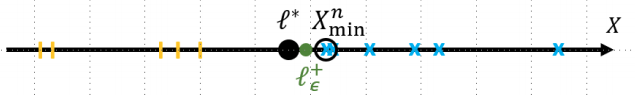
\includegraphics[width=\columnwidth]{Resources/pac-halfline}
\end{center}
If $l_\epsilon^+ \leq X_{\textit{min}}^n$: $l^*\leq X_i \leq X_{\textit{min}}^n$.

Then $\mathcal R(\hat c_n) = \P(l^*\leq X_i \leq X_{\textit{min}}^n)$ ${\color{imp}\geq} \P(l^*\leq X_i \leq l_\epsilon^+) = \epsilon$

$\P(l_\epsilon^+\leq X_{\textit{min}}^n) = \prod_i^n \P[X_i\not\in[l^*, l_\epsilon^+)] = \prod(1 - \P(l^*\leq X_i \leq l_\epsilon^+)) = (1-\epsilon)^n$

$\P(\mathcal R(\hat c_n)\geq \epsilon) = \P(l_\epsilon^+\leq X_{\textit{min}}^n)$ 
$= (1-\epsilon)^n {\color{imp} \leq \delta}$. $\to n \geq \frac{1}{\epsilon}\log\frac{1}{\delta}$.

%\subsubsection{The general PAC model}
%A learning algorithm $\mathcal A$ can learn a concept class $\mathcal C$ from $\mathcal H$ if given {\color{imp3}sufficiently large sample} as input, outputs a hypothesis that \textbf{{\color{imp}generalizes well} {\color{imp2}with high probability}}
%
%\textbf{Definition: } A learning algorithm $\mathcal A$ can learn a concept class $\mathcal C$ from $\mathcal H$ if there is a {\color{imp3} polynomial function $\mathit{poly}$}, such that
%\begin{enumerate}
%	\item For any distribution $\mathcal D$ on $\mathcal X\times \{0,1\}$ and
%	\item for any {\color{imp}$0<\epsilon<1/2$} and {\color{imp2}$0<\delta<1/2$}
%\end{enumerate}
%if $\mathcal A$ receives as input {\color{imp3} a sample $\mathcal Z$ of size $n\geq \mathit{poly}(1/\epsilon, 1/\delta, \mathit{dim}(\mathcal X)$}, then $\mathcal A$ outputs $\hat c\in\mathcal H$, sucht that
%$
%	{\color{imp2}\P_{\mathcal Z\sim \mathcal D^n}\left({\color{imp}\mathcal R(\hat c) - \inf_{c\in\mathcal C}\mathcal R(c)\leq \epsilon }\right) \geq 1 - \delta}
%$
%

\end{multicols*}
\end{document}